\section{Integration}
To be able to simulate the particles with more precision, we have implemented multiple integration schemes. This has been done, since the euler method is very unstable and can explode very fast. Therefore we have implemented the following integration schemes:
\begin{itemize}
  \item[-] Euler
  \item[-] Mid-Point
  \item[-] Runge-Kutta 4-order
\end{itemize}
The difference of the integration schemes can be notices easily. As displayed below, the Runga Kutta method is more stable than euler.

\begin{figure}[!htbp]
  \begin{subfigure}[h]{\textwidth}
  \centering
    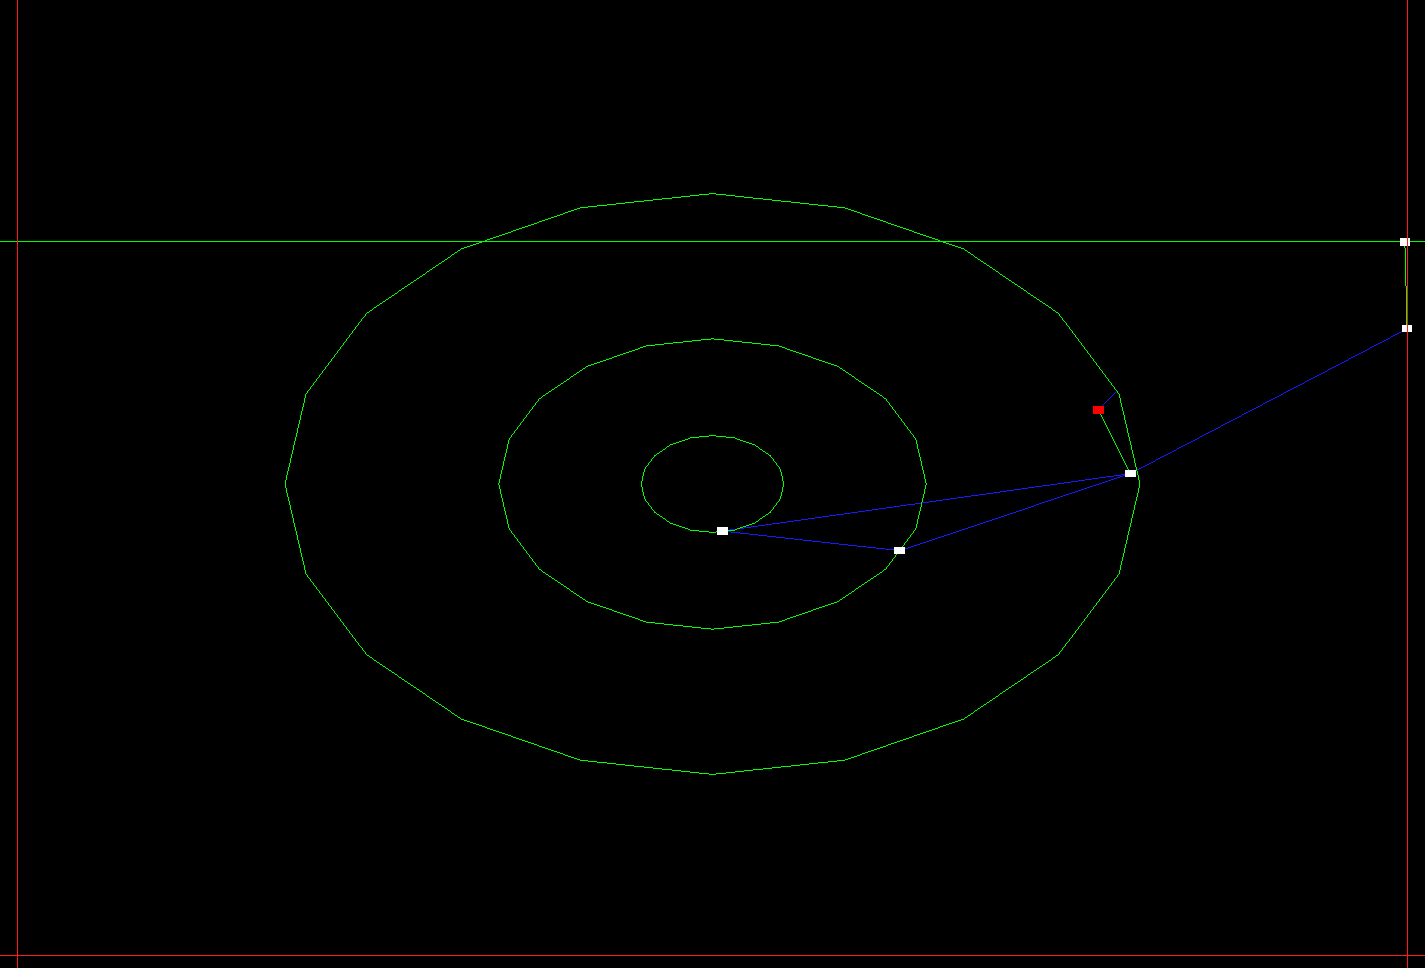
\includegraphics[width=0.3\textwidth]{euler1}
    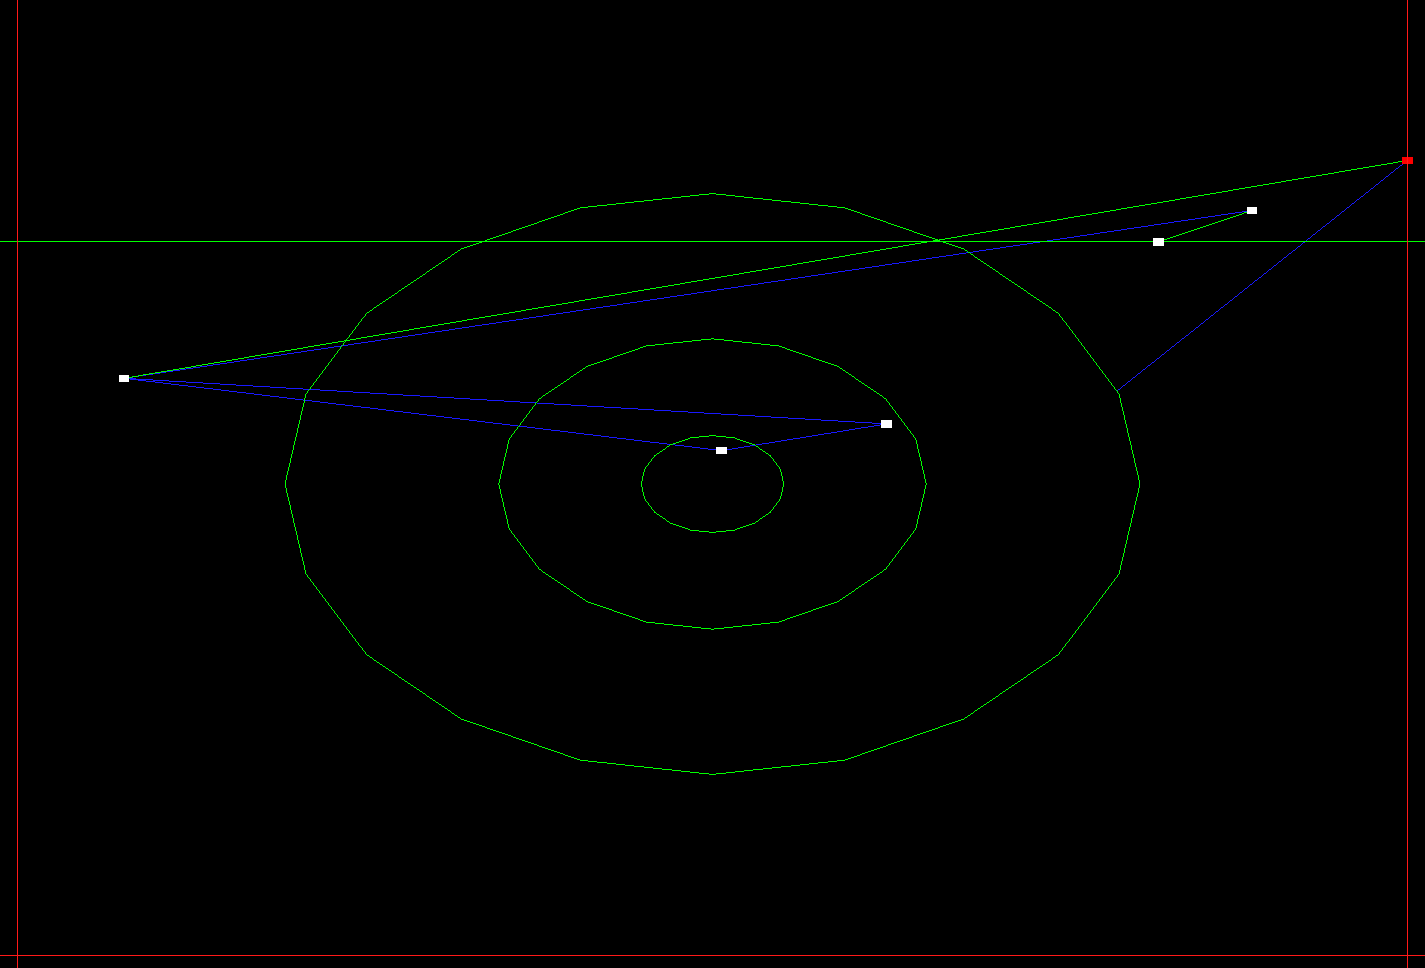
\includegraphics[width=0.3\textwidth]{euler2}
    \caption{Euler integration explodes after short time at time-step 0.02s}
    \label{fig:euler}
  \end{subfigure}
  \\
  \begin{subfigure}[h]{\textwidth}
  \centering
    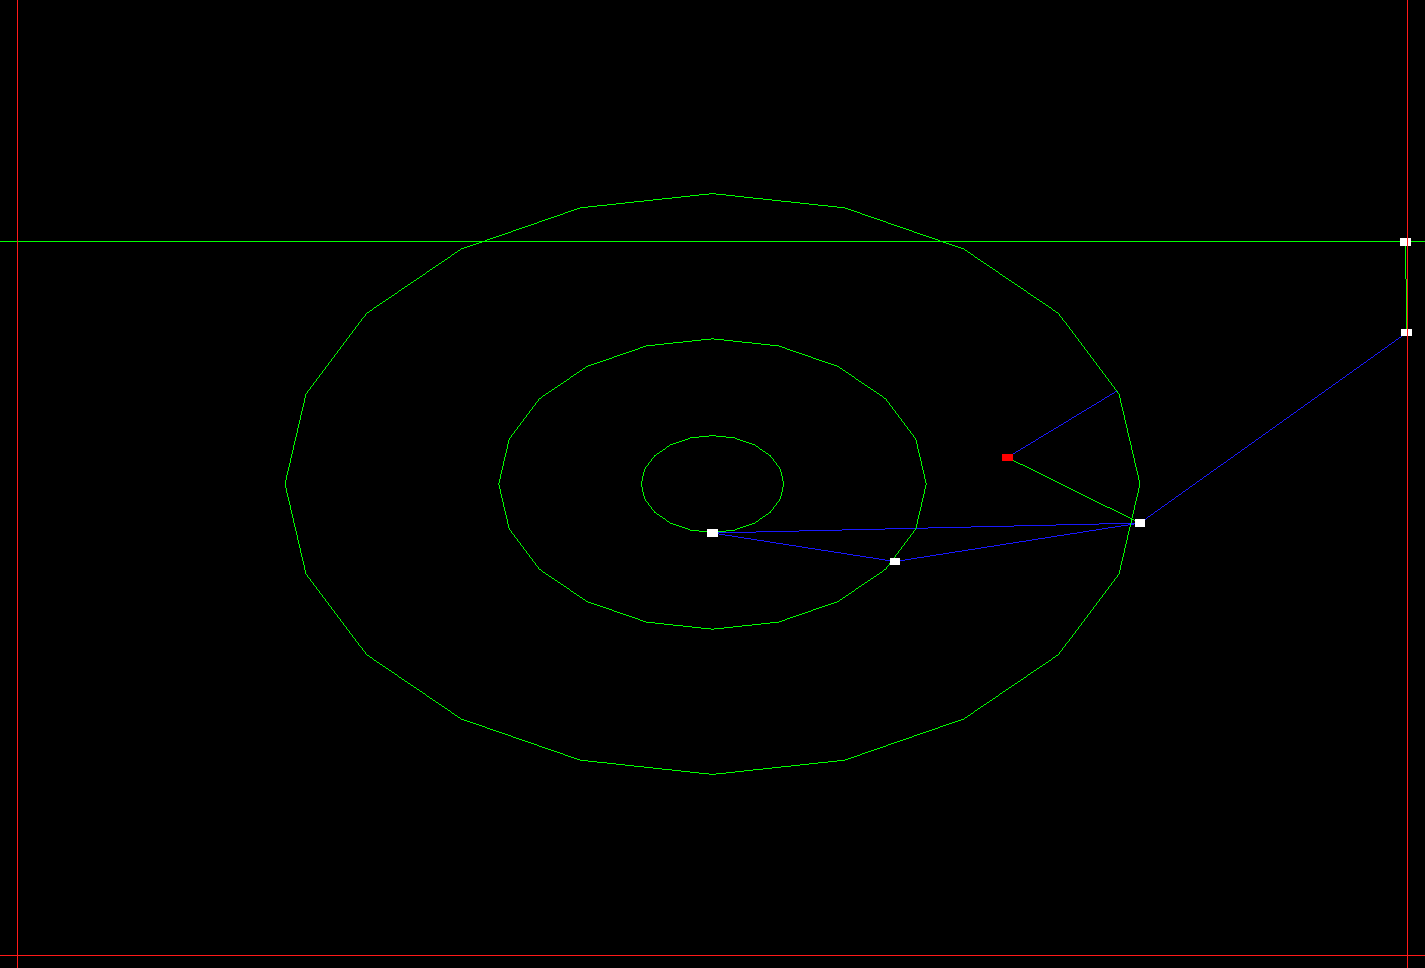
\includegraphics[width=0.3\textwidth]{runga1}
    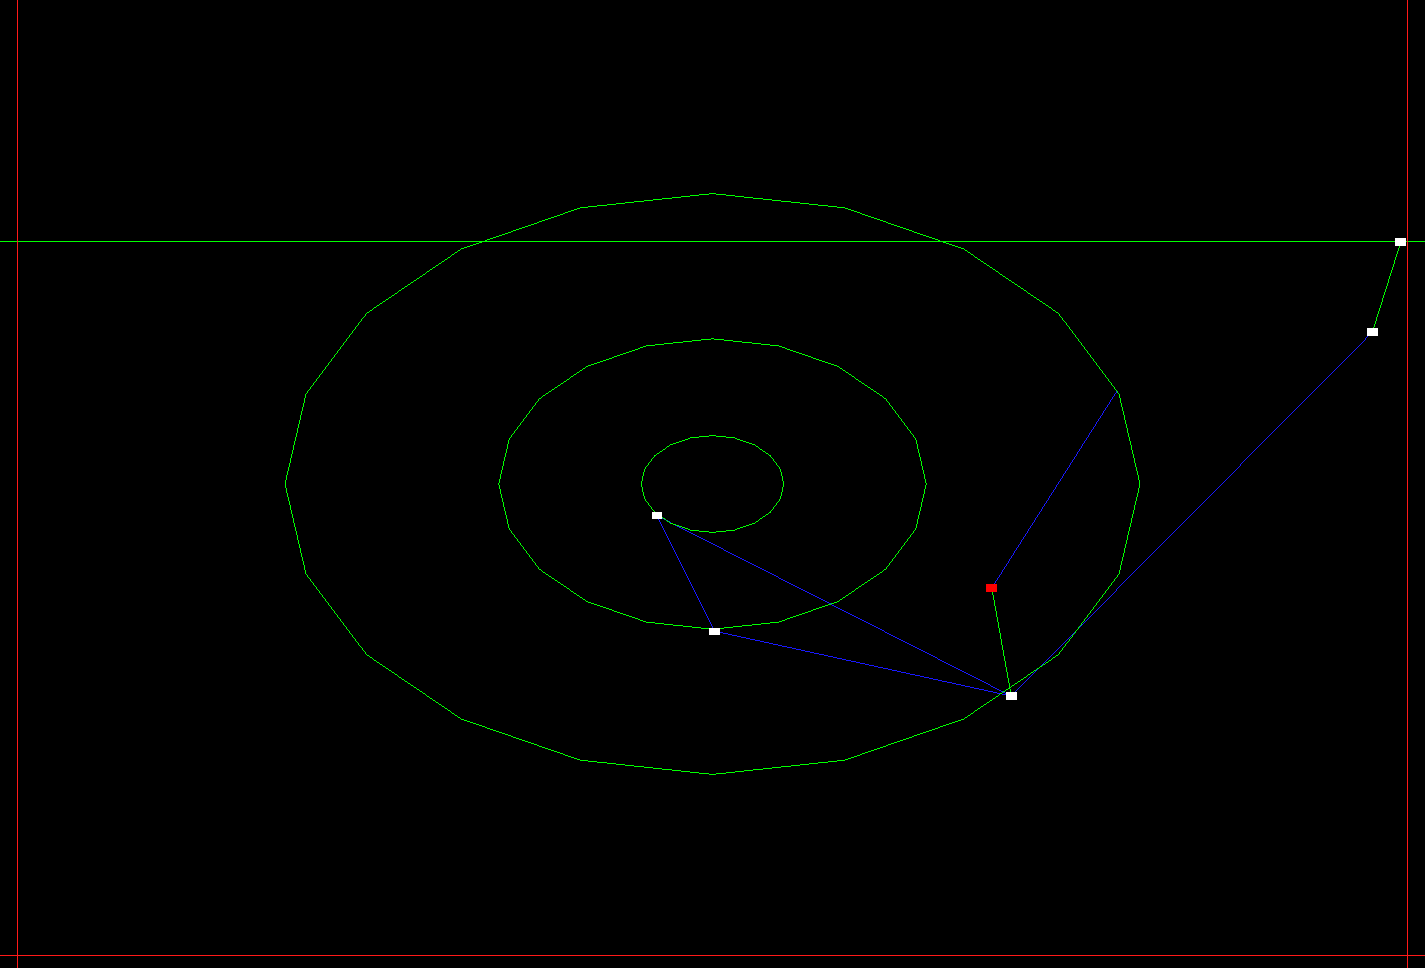
\includegraphics[width=0.3\textwidth]{runga2}
    \caption{Runga Kutta integration stays stable at time-step 0.02s}
    \label{fig:ruga}
  \end{subfigure}
  
  \caption{Comparison Euler and Runga Kutta integration scheme}
  \label{fig:integration}
\end{figure}
